 %
% teil1.tex -- Beispiel-File für das Paper
%
% (c) 2020 Prof Dr Andreas Müller, Hochschule Rapperswil
%
% !TEX root = ../../buch.tex
% !TEX encoding = UTF-8
%
\section{Metrischer Tensor
\label{geodaeten:section:MetrischerTensor}}
\rhead{Der Metrische Tensor}

Im vorherigen Kapitel wurde das Konzept des Linienelements erläutert.
Es wurde aufgezeigt, wie dieses mittels geometrischer Analyse für verschiedene Räume und Koordinatensysteme berechnet werden kann.
Aus der Vektorgeometrie ist uns jedoch ein anderes nützliches Werkzeug bekannt, welches uns erlaubt, Abstände in einem Raum zu berechnen: Das Skalarprodukt.

\subsection{Skalarprodukt im euklidischen Raum}
Im euklidischen Raum ist das Skalarprodukt zwischen zwei Vektoren $\vec{u}$ und $\vec{v}$ definiert als
\begin{equation}
	\vec{u} \cdot \vec{v} = \sum_{i=1}^n u_i v_i,
\end{equation}
wobei $\vec{u} = (u_1, u_2, \ldots, u_n)$ und $\vec{v} = (v_1, v_2, \ldots, v_n)$ die Komponenten der Vektoren in einem $n$-dimensionalen Raum sind.

Die Länge eines Vektors $\vec{u}$ ergibt sich als die Wurzel aus dem Skalarprodukt des Vektors mit sich selbst, also
\begin{equation}
	\|\vec{u}\| = \sqrt{\vec{u} \cdot \vec{u}} = \sqrt{\sum_{i=1}^n u_i^2}.
\end{equation}

Betrachten wir nun einen infinitesimal kleinen Vektor in einer Ebene mit kartesischen Koordinaten $(x, y)$, dann ergibt das Skalarprodukt dieses Vektors mit sich selbst
\begin{equation}
	ds^2 = dx \cdot dx + dy \cdot dy = dx^2 + dy^2,
\end{equation}
was die quadratische infinitesimale Länge des Vektors beschreibt und dem bereits bekannten Linienelement entspricht.

Diese Definition des Skalarprodukts ist jedoch nicht allgemeingültig und gilt nur für die Berechnung von Abständen im euklidischen Raum.
Für komplexere Räume mit speziellen Koordinatensystemen wie Zylinder- oder Kugelkoordinaten müssen wir zuerst die Konzepte der Mannigfaltigkeit und des metrischen Tensors verstehen.

\subsection{Mannigfaltigkeit}
Eine Mannigfaltigkeit ist ein mathematisches Konstrukt, das dazu dient, komplizierte geometrische Objekte in eine einfachere, lokal verständliche Form zu bringen.
Im Wesentlichen ist eine Mannigfaltigkeit eine Sammlung von Punkten, die den Raum in lokal euklidische Bereiche unterteilt. 

Ein einfaches Beispiel hierfür ist die Erdoberfläche.
Steht ein ``Flat-Earther" auf der Erdoberfläche, so erscheint ihm die Erde flach, weil der Bereich, den er betrachtet, sehr klein ist im Vergleich zur Gesamtgröße der Erde.
Würde dieser ``Flat-Earther" jedoch weiter zurücktreten und die gesamte Erde betrachten, sollte auch er erkennen können, dass sie in Wirklichkeit eine Kugel ist.

Eine Mannigfaltigkeit ist also ein mathematisches Objekt, das lokal flach oder euklidisch erscheint, aber global eine kompliziertere Struktur haben kann, wie zum Beispiel die Oberfläche einer Kugel.

Eine differenzierbare Mannigfaltigkeit setzt zusätzlich voraus, dass sie in der Umgebung jedes Punktes lokal differenzierbar ist, wodurch die Mannigfaltigkeit eine glatte Struktur erhält.
Da sich die Mannigfaltigkeit lokal wie ein differenzierbarer euklidischer Raum verhält, ermöglicht uns das, für jeden Punkt ein Skalarprodukt zu definieren.
Die Funktion, die das Skalarprodukt für jeden Punkt einer solchen Mannigfaltigkeit definiert, wird als Metrik bezeichnet.

\begin{figure}
	\centering
	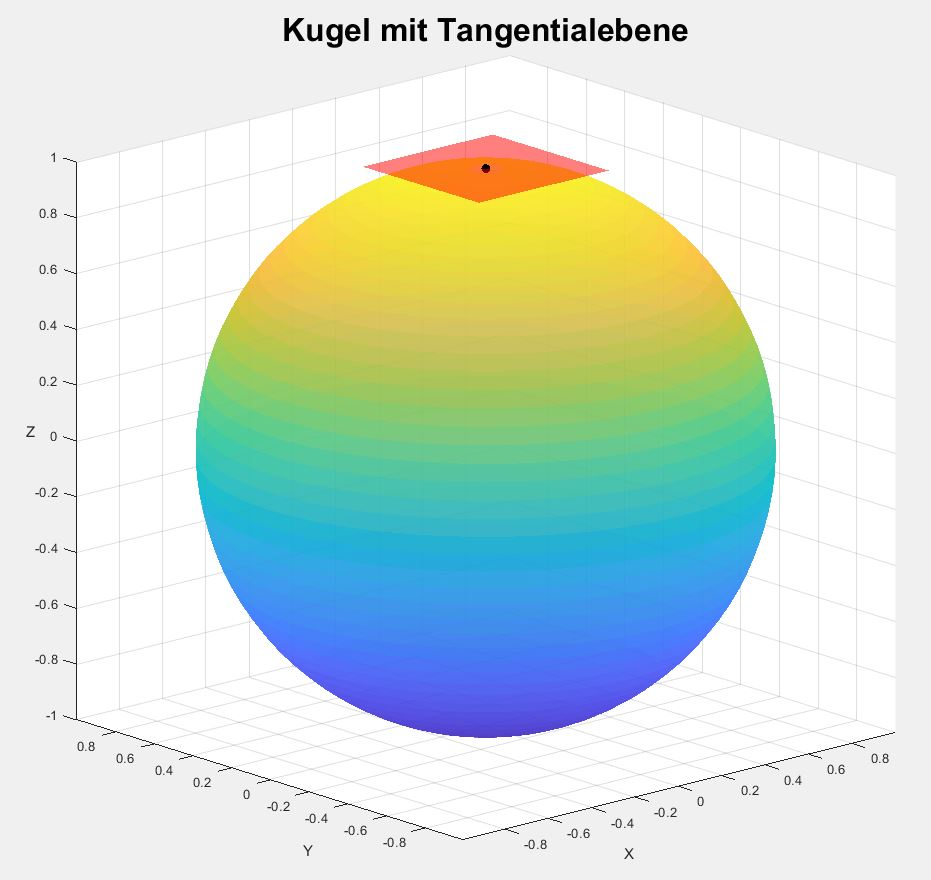
\includegraphics[width=1\linewidth]{papers/geodaeten/Abbildungen/MetrischerTensor/Tangentialebene}
	\caption{Tangentialebene eines Punktes der riemannschen Mannigfaltigkeit einer Kugeloberfläche}
	\label{geodaeten:figure:MetrischerTensor:Tangentialebene}
\end{figure}

\subsection{Metrik und metrischer Tensor}
Die Metrik ist das grundlegende Werkzeug, welches uns ermöglicht, Längen, Abstände und Winkel in einem Raum zu messen.
In einfachen geometrischen Räumen, wie dem euklidischen Raum, kennen wir die Metrik bereits als den Satz des Pythagoras.
Wir haben auch schon in Abschnitt \ref{geodaeten:section:Linienelemente:Beispiele} die Metrik in verschiedenen Koordinatensystemen angewendet, um Linienelemente auf unterschiedlichen Oberflächen zu berechnen.

Um die Metrik mathematisch darstellen zu können wird der metrische Tensor $g_{ij}$ eingeführt.
Dieser Tensor ist eine symmetrische $n \times n$-Matrix, wobei $n$ der Dimension des Raumes entspricht, die die Metrik an jedem Punkt der Mannigfaltigkeit kodiert.
Er enthält alle Informationen darüber, wie Abstände und Winkel in einem Raum berechnet werden.
Auf diese Weise beschreibt der metrische Tensor die geometrische Struktur des gesamten Raumes.

Eine differenzierbare Mannigfaltigkeit, die an jedem Punkt durch einen metrischen Tensor definiert ist, wird als Riemannsche Mannigfaltigkeit bezeichnet. Zusätzlich erfordert eine Riemannsche Mannigfaltigkeit, dass der metrische Tensor selbst stetig differenzierbar und ausserdem noch positiv definit ist. 
Dies bedeutet, dass in Riemannschen Mannigfaltigkeiten kein negativer Abstand existieren kann.

Mit dem metrischen Tensor kann ein allgemeines, von Koordinatensystemen unabhängiges Skalarprodukt zweier Vektoren $\vec{u}$ und $\vec{v}$ definiert werden als
\begin{equation}
	\vec{u} \cdot \vec{v} = g_{ij} \, u^i \, v^j.
\end{equation}
Die Notation des metrischen Tensors stammt aus der Tensoralgebra,
wobei die einsteinsche Summenkonvention eine Summierung über die Indizes $i$ und $j$ impliziert, welche die Dimensionen des Raumes durchlaufen.
Die Komponenten der Vektoren $u^i$ und $v^j$ werden dabei durch den metrischen Tensor $g_{ij}$ gewichtet, wodurch sich eine Summe in der Form von
\begin{equation}
	g_{11} \, u_1 \, v_1 + g_{12} \, u_1 \, v_2 + \dots + g_{nn} \, u_n \, v_n
\end{equation}
ergibt.
Berechnet man nun mit dieser allgemeinen Definition das Skalarprodukt eines infinitesimalen Vektors mit sich selbst, erhält man
\begin{equation}
	ds^2 = g_{ij} \, du^i \, du^j.
	\label{geodaeten:equation:MetrischerTensor:AllgemeinesLinienelement}
\end{equation}
Somit lässt sich das Linienelement in einer allgemeinen Form ausdrücken, die mithilfe des metrischen Tensors zu einer koordinatenunabhängigen Funktion wird.

Der metrische Tensor ist daher von zentraler Bedeutung für das Verständnis der Geometrie eines Raumes und ist ein fundamentales Werkzeug in der Differentialgeometrie und der allgemeinen Relativitätstheorie. 
Er ermöglicht es uns, die Metrik eines Raumes in eine kompakte Schreibweise zu überführen und liefert die Grundlage für die Berechnung von Abständen und Winkeln in komplexeren geometrischen Strukturen.

Im nächsten Abschnitt werden wird anhand von Beispielen gezeigt, wie die Metrik von verschiedenen Koordinatensystemen, in die kompakte Form des metrischen Tensors überführt werden kann.

\section{Beispiele zum metrischen Tensor}

%
% teil1.tex -- Beispiel-File für das Paper
%
% (c) 2020 Prof Dr Andreas Müller, Hochschule Rapperswil
%
% !TEX root = ../../buch.tex
% !TEX encoding = UTF-8
%
\subsection{Kartesisch\label{geodaeten:section:MetrischerTensor:Kartesisch}}
\rhead{Metrischer Tensor Beispiele}

Der Metrische Tensor für einen zweidimensionalen kartesischen Raum kann aus der Gleichung \eqref{geodaeten:equation:MetrischerTensor:AllgemeinesLinienelement} des allgemeinen Linienelements hergeleitet werden.
Schreiben wir die einsteinsche-Summe für zwei Dimensionen aus ergibt sich
\begin{equation}
	ds^2 = g_{11}  du^1  du^1 + g_{12}  du^1  du^2 + g_{21}  du^2  du^1 + g_{22}  du^2  du^2 .
	\label{geodaeten:equation:MetrischerTensor:Kartesisch:EinsteinSumme}
\end{equation}

In dem kartesischen Raum gilt, $du^1 = dx$ und $du^2 = dy$ wobei zu beachten ist, dass bei der Einsteinschen Summenkonvention die Hochstele keiner Potenz sondern eines Index entspricht.
Aus Abschnitt \ref{geodaeten:section:Linienelemente:Kartesisch} kennen wir das Linienelement des Kartesischen Raums als

\begin{equation}
	ds^2 = dx^2 + dy^2 .
\end{equation}
Aus dem Linienelement können wir die Koeffizienten von 

\begin{equation}
du^1 du^1 = dx^2 \quad \text{und} \quad du^2  du^2 = dy^2 
\end{equation}
als $1$ herauslesen.
Die Koeffizienten für

\begin{equation}
du^1 \cdot du^2 = dx \cdot dy \quad \text{und} \quad du^2 \cdot du^1 = dy \cdot dx
\end{equation}
sind beide $0$.
In Gleichung \ref{geodaeten:equation:MetrischerTensor:Kartesisch:EinsteinSumme} ist zu erkennen, dass diese Koeffizienten den Werten im metrischen Tensor $g_{ij}$ entsprechen.
An den richtigen Stellen eingesetzt ergibt sich der metrische Tensor des kartesischen Raums zu

\begin{equation}
	\begin{aligned}
		g_{11} &= \textcolor{red}{1} \\
		g_{12} &= \textcolor{blue}{0} \\
		g_{21} &= \textcolor{darkgreen}{0} \\
		g_{22} &= \textcolor{magenta}{1} \\
		g_{ij} &= \begin{pmatrix} \textcolor{red}{1} && \textcolor{blue}{0} \\ \textcolor{darkgreen}{0} && \textcolor{magenta}{1} \end{pmatrix} .
	\end{aligned}
\end{equation}


%
% teil1.tex -- Beispiel-File für das Paper
%
% (c) 2020 Prof Dr Andreas Müller, Hochschule Rapperswil
%
% !TEX root = ../../buch.tex
% !TEX encoding = UTF-8
%
\subsection{Zylinder\label{geodaeten:section:MetrischerTensor:Zylinder}}
\rhead{Metrischer Tensor Beispiele}

Für die Zylinderoberfläche gilt $r$ als konstant und $u^1 = \phi$, $u^2 =z$ 
Vergleicht man die Einstein-Summe aus Gleichung \eqref{geodaeten:equation:MetrischerTensor:Kartesisch:EinsteinSumme} mit dem Linienelement der Zylinderoberfläche

\begin{equation}
	\begin{aligned}
	ds^2 &= g_{11} \cdot du^1 \cdot du^1 + g_{12} \cdot du^1 \cdot du^2 + g_{21} \cdot du^2 \cdot du^1 + g_{22} \cdot du^2 \cdot du^2 \\
	&= r^2 \cdot d \phi^2 +dz^2
	\end{aligned}
\end{equation}
Kann mittels Koeffizienten Vergleich bestimmt werden, dass 

\begin{equation}
	\begin{alignedat}{3}
		g_{11} \cdot du^1 \cdot du^1 &= g_{11} \cdot d \phi^2 & &= r^2 \cdot d \phi^2 \\
		g_{22} \cdot du^2 \cdot du^2 &= g_{22} \cdot dz^2    & &= 1 \cdot dz^2 \\
		g_{12} \cdot du^1 \cdot du^2 &= g_{12} \cdot d \phi \cdot dz & &= 0 \cdot d \phi \cdot dz \\
		g_{21} \cdot du^2 \cdot du^2 &= g_{21} \cdot dz \cdot d \phi & &= 0 \cdot dz \cdot d \phi .
	\end{alignedat}
\end{equation}
Die Matrixeinträge entsprechen den Koeffizienten der jeweiligen Ableitungsprodukte und damit lässt sich der metrische Tensor aufstellen als
\begin{equation}
	g_{ji} =\begin{pmatrix} g_{11} && g_{12} \\ g_{21} && g_{22} \end{pmatrix}= \begin{pmatrix} r^2 && 0 \\ 0 && 1 \end{pmatrix} .
\end{equation}

Ist $r$ nicht konstant, bedeutet dies, dass man sich in drei Dimensionen bewegen kann.
Deshalb muss eine $3 \times 3$-Matrix für den metrischen Tensor entstehen, damit jede Bewegung vollständig beschrieben ist. 

Die Einstein-Summe hat hier die Form

\begin{equation}
\begin{aligned}
	ds^2 = &\ g_{11} \cdot du^1 \cdot du^1 + g_{12} \cdot du^1 \cdot du^2 + g_{13} \cdot du^1 \cdot du^3 \nonumber \\
	&+ g_{21} \cdot du^2 \cdot du^1 + g_{22} \cdot du^2 \cdot du^2 + g_{23} \cdot du^2 \cdot du^3 \nonumber \\
	&+ g_{31} \cdot du^3 \cdot du^1 + g_{32} \cdot du^3 \cdot du^2 + g_{33} \cdot du^3 \cdot du^3  .
\end{aligned} 
	\label{geodaeten:equation:MetrischerTensor:Kartesisch:EinsteinSumme3D}
\end{equation}

Im Linienelement des Zylinders aus \eqref{geodaeten:equation:Linienelemente:Zylinder:Zylinder3D} kann man herauslesen, dass keine Terme mit gemischten Ableitungsprodukte vorhanden sind.
Daher sind alle Einträge außer den Diagonalen Null.
Mit $u^1 = r$, $u^2 = \phi$ und $u^3 = z$  können die diagonalen Elemente mit den Koeffizienten im Linienelement bestimmt werden. 
Somit gilt,

\begin{equation}
	\begin{aligned}
		g_{11}  &= 1  \\
		g_{22}  &= r^2 \\
		g_{33}  &= 1  
	\end{aligned}
\end{equation}
und damit ist der metrische Tensor im dreidimensionalen zylindrischen Raum

\begin{equation}
	T = \begin{pmatrix} 1 && 0 && 0 \\ 0 && r^2 && 0 \\ 0 && 0 && 1 \end{pmatrix} .
\end{equation}

Dieses Beispiel veranschaulicht, dass der metrische Tensor eine $n \times n$-Matrix ist, wobei $n$ der Anzahl Dimensionen entspricht.
Dieser metrische Tensor beinhaltet eine Variable $r$ und ist somit nicht konstant. 
Daher existiert für die dreidimensionale Oberfläche des vierdimensionalen zylindrischen Raums eine Krümmung.
Diese Krümmung eines vierdimensionalen Raums ist allerdings schwer vorzustellen, weshalb die Krümmung des metrischen Tensors im Beispiel der Kugel (Abschnitt \ref{geodaeten:section:MetrischerTensor:Kugel}) genauer vorgestellt wird.

%
% teil1.tex -- Beispiel-File für das Paper
%
% (c) 2020 Prof Dr Andreas Müller, Hochschule Rapperswil
%
% !TEX root = ../../buch.tex
% !TEX encoding = UTF-8
%
\subsection{Kugel\label{geodaeten:section:MetrischerTensor:Kugel}}
\rhead{Metrischer Tensor Beispiele}

Sed ut perspiciatis unde omnis iste natus error sit voluptatem
accusantium doloremque laudantium, totam rem aperiam, eaque ipsa
quae ab illo inventore veritatis et quasi architecto beatae vitae
dicta sunt explicabo.
Nemo enim ipsam voluptatem quia voluptas sit aspernatur aut odit
aut fugit, sed quia consequuntur magni dolores eos qui ratione
voluptatem sequi nesciunt




